%%%%%%%%%%%%%%%%%%%%%%%%%%%%%%%%%%%%%%%%%
% Beamer Presentation
% LaTeX Template
% Version 1.0 (10/11/12)
%
% This template has been downloaded from:
% http://www.LaTeXTemplates.com
%
% License:
% CC BY-NC-SA 3.0 (http://creativecommons.org/licenses/by-nc-sa/3.0/)
%
%%%%%%%%%%%%%%%%%%%%%%%%%%%%%%%%%%%%%%%%%

%----------------------------------------------------------------------------------------
%	PACKAGES AND THEMES
%----------------------------------------------------------------------------------------

\documentclass{beamer}

\mode<presentation> {

% The Beamer class comes with a number of default slide themes
% which change the colors and layouts of slides. Below this is a list
% of all the themes, uncomment each in turn to see what they look like.

%\usetheme{default}
%\usetheme{AnnArbor}
%\usetheme{Antibes}
%\usetheme{Bergen}
%\usetheme{Berkeley}
%\usetheme{Berlin}
%\usetheme{Boadilla}
%\usetheme{CambridgeUS}
%\usetheme{Copenhagen}
%\usetheme{Darmstadt}
%\usetheme{Dresden}
%\usetheme{Frankfurt}
\usetheme{Goettingen}	% vpravo
%\usetheme{Hannover}
%\usetheme{Ilmenau}
%\usetheme{JuanLesPins}
%\usetheme{Luebeck}
%\usetheme{Madrid}
%\usetheme{Malmoe}			
%\usetheme{Marburg}
%\usetheme{Montpellier}
%\usetheme{PaloAlto}
%\usetheme{Pittsburgh}
%\usetheme{Rochester}
%\usetheme{Singapore}			
%\usetheme{Szeged}
%\usetheme{Warsaw}

% As well as themes, the Beamer class has a number of color themes
% for any slide theme. Uncomment each of these in turn to see how it
% changes the colors of your current slide theme.

%\usecolortheme{albatross}
%\usecolortheme{beaver}
%\usecolortheme{beetle}
%\usecolortheme{crane}
%\usecolortheme{dolphin}
%\usecolortheme{dove}
%\usecolortheme{fly}
%\usecolortheme{lily}			
%\usecolortheme{orchid}
%\usecolortheme{rose}
%\usecolortheme{seagull}
%\usecolortheme{seahorse}
%\usecolortheme{whale}
%\usecolortheme{wolverine}

%\setbeamertemplate{footline} % To remove the footer line in all slides uncomment this line
%\setbeamertemplate{footline}[page number] % To replace the footer line in all slides with a simple slide count uncomment this line

%\setbeamertemplate{navigation symbols}{} % To remove the navigation symbols from the bottom of all slides uncomment this line
}

\usepackage[utf8]{inputenc}	% kódování textu
\usepackage[czech]{babel}		% zavedení češtiny
\usepackage{amsmath,amsfonts,amssymb}	% matematika
\usepackage{graphicx} % Allows including images
\usepackage{booktabs} % Allows the use of \toprule, \midrule and \bottomrule in tables
\usepackage{multirow}	% slouceni radek v tabulce
\usepackage{multicol}	% slouceni sloupcu v tabulce
\usepackage{longtable}	% rozdeleni tabulky pres vice stran
\usepackage{enumerate}	% seznamy
\usepackage{float}
\usepackage{lscape}		% stranka na sirku
\usepackage{fancyhdr}
\usepackage{url}
\usepackage{array}
\usepackage{subfigure}
\usepackage{dirtree}
\usepackage{setspace}
\usepackage{color}
\usepackage{listings}
\usepackage{multimedia}


%------------------------------------------------------------------
%	TITLE PAGE
%------------------------------------------------------------------

\title[]{Zásuvný modul QGIS pro~zpracování přípravné fáze komplexních pozemkových úprav} % The short title appears at the bottom of every slide, the full title is only on the title page

\author{Bc. Ondřej Svoboda} % Your name
\institute[ČVUT] % Your institution as it will appear on the bottom of every slide, may be shorthand to save space
{
České vysoké učení technické v Praze \\ % Your institution for the title page
%\medskip
Fakulta stavební \\
%\medskip
Obor Geomatika
% \textit{ondrej.svoboda.2@fsv.cvut.cz} % Your email address
}
\date{22. června 2017} % Date, can be changed to a custom date
\titlegraphic{
\includegraphics[width=1.5cm]{pictures/logo2.pdf}}

\begin{document}

\begin{frame}
\titlepage % Print the title page as the first slide
\end{frame}

\begin{frame}
\frametitle{Obsah} % Table of contents slide, comment this block out to remove it
\tableofcontents % Throughout your presentation, if you choose to use \section{} and \subsection{} commands, these will automatically be printed on this slide as an overview of your presentation
\end{frame}

%------------------------------------------------------------------
%	PRESENTATION SLIDES
%------------------------------------------------------------------

%------------------------------------------------------------------
\section{Motivace} % Sections can be created in order to organize your presentation into discrete blocks, all sections and subsections are automatically printed in the table of contents as an overview of the talk
%------------------------------------------------------------------

\begin{frame}

\frametitle{Motivace}

Význam pozemkových úprav
\begin{itemize}
	\item zlepšení podmínek pro zemědělské hospodaření
	\item zpřístupnění pozemků
	\item zmírnění účinků vodní a~větrné eroze
	\item zlepšení životního prostředí
	\item zvýšení ekologické stability krajiny
	\item vyjasnění vlastnických vztahů
\end{itemize}

\bigskip

Běžně používané programy
\begin{itemize}
	\item proprietární software
	\item pouze pro platformu Microsoft Windows
\end{itemize}

\end{frame}

%------------------------------------------------------------------

\section{Zadání}

\begin{frame}

\frametitle{Zadání}

\begin{itemize}
	\item zásuvný modul programu QGIS
	\item přípravná fáze komplexních pozemkových úprav
	\item práce a~editace dat ve formátu VFK
	\item rozdělení parcel do kategorií
	\item nástroje pro kontrolu souladu SPI a~SGI
	\item oceňování podle BPEJ
\end{itemize}

\end{frame}

%------------------------------------------------------------------

\section{Teoretický úvod}

\subsection{Pozemkové úpravy} % A subsection can be created just before a set of slides with a common theme to further break down your presentation into chunks

\begin{frame}

\frametitle{Pozemkové úpravy}

Formy pozemkových úprav
\begin{itemize}
	\item jednoduché pozemkové úpravy
	\item komplexní pozemkové úpravy
\end{itemize}

\bigskip

Obvod pozemkových úprav
\begin{itemize}
	\item území dotčené pozemkovými úpravami
\end{itemize}

\bigskip

Předmět pozemkových úprav
\begin{itemize}
	\item pozemky v~obvodu řešené dle § 2 zákona č.~139/2002
	\item pozemky v~obvodu neřešené dle § 2 zákona č.~139/2002
	\item pozemky mimo obvod
\end{itemize}

\end{frame}

%------------------------------------------------------------------

\begin{frame}

\frametitle{Přípravná fáze}

\begin{itemize}
	\item určení obvodu
	\item zjišťování průběhu hranic
	\item vstupní soupisy nároků vlastníků
	\begin{itemize}
		\item kontrola souladu SPI a~SGI
		\item výpočet opravného koeficientu dle zaměření skutečného stavu
		\item ocenění pozemků
		\item výpočet vzdálenosti pozemků
		\item prosté nároky ve~výměře a~ceně
		\item průměrná vzdálenost pozemků
		\item upravené nároky ve~výměře a~ceně
	\end{itemize}
\end{itemize}

\end{frame}

%------------------------------------------------------------------

\subsection{VFK}

\begin{frame}

\frametitle{VFK}

\begin{itemize}
	\item SPI i~SGI
	\item vzájemné předávání dat mezi informačním systémem katastru nemovitostí a jinými systémy
	\item textový soubor s příponou \textit{*.vfk}
	\item struktura
	\begin{itemize}
		\item hlavička – řádky uvozené \texttt{\&H}
		\item datové bloky – řádky uvozené \texttt{\&B} a \texttt{\&D}
		\item koncový znak – znak \texttt{\&K}
	\end{itemize}
\end{itemize}

\end{frame}

%------------------------------------------------------------------

\subsection{BPEJ}

\begin{frame}

\frametitle{BPEJ}

\begin{itemize}
	\item vyjadřuje produkční potenciál zemědělské půdy
	\item spravuje Státní pozemkový úřad
	\item celostátní databáze od dubna 2017 veřejně dostupná
	\item pětimístný kód BPEJ
\end{itemize}

\end{frame}

%------------------------------------------------------------------

\section{Použité technologie}

\begin{frame}

\frametitle{Použité technologie}

\begin{figure}
	\centering
	\begin{minipage}{.4\textwidth}
		\centering
		\visible<1->{
		\begin{figure}[ht]
	  		
\includegraphics[width=2.5cm]{pictures/qgis_logo.png}
		\end{figure}}
    \end{minipage}%
    \begin{minipage}{.6\textwidth}
		\centering
		\visible<2->{
		\begin{figure}[ht]
			
\includegraphics[width=6cm]{pictures/python_logo.png}
		\end{figure}}
	\end{minipage}
\end{figure}

\begin{figure}
	\centering
	\begin{minipage}{.32\textwidth}
		\centering
		\visible<3->{
		\begin{figure}[ht]
	  		
\includegraphics[width=2.5cm]{pictures/sqlite_logo.png}
		\end{figure}}
    \end{minipage}%
    \begin{minipage}{.32\textwidth}
		\centering
		\visible<4->{
		\begin{figure}[ht]
			
\includegraphics[width=1.5cm]{pictures/pyqt_logo.png}
		\end{figure}}
	\end{minipage}
    \begin{minipage}{.32\textwidth}
		\centering
		\visible<5->{
		\begin{figure}[ht]
			
\includegraphics[width=2cm]{pictures/gdal_logo.png}
		\end{figure}}
	\end{minipage}
\end{figure}

\end{frame}

%------------------------------------------------------------------

\section{Zásuvný modul}

\subsection{Grafické uživatelské rozhraní}

\begin{frame}

\frametitle{Grafické uživatelské rozhraní}

\begin{itemize}
	\item v českém jazyce
	\begin{itemize}
		\item legislativa České republiky
		\item VFK
	\end{itemize}
\end{itemize}

\begin{figure}[ht]
	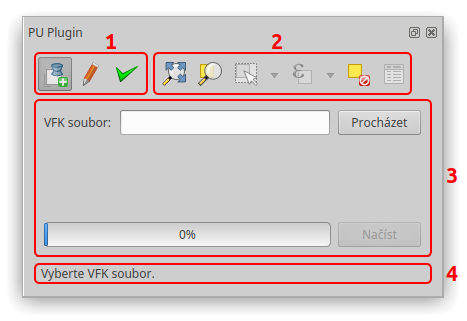
\includegraphics[width=0.6\textwidth]{pictures/main_gui.png}
\end{figure}

\end{frame}

%------------------------------------------------------------------

\subsection{Načtení VFK souboru}

\begin{frame}

\frametitle{Načtení VFK souboru}

\begin{itemize}
	\item VFK soubor – tabulka \texttt{PAR}
	\item knihovna GDAL
	\begin{itemize}
		\item VFK Driver
		\item SQLite Driver
		\begin{itemize}
			\item \texttt{\detokenize{geometry_columns}}
			\item \texttt{\detokenize{spatial_ref_sys}}
		\end{itemize}
	\end{itemize}
	\item přidání vlastních sloupců
	\item OGR poskytovatel dat nepoužíval transakce
	\item symbologie podle QML souboru
	\item atributová tabulka s aliasy
\end{itemize}

\begin{figure}[ht]
	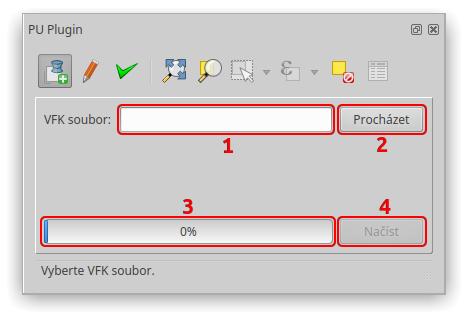
\includegraphics[width=0.55\textwidth]{pictures/nacteni_vfk_gui.png}
\end{figure}

\end{frame}

%------------------------------------------------------------------

\subsection{Editace}

\begin{frame}

\frametitle{Editace}

\begin{itemize}
	\item určení obvodu pozemkové úpravy a rozdělení parcel do kategorií
	\item vrstva \texttt{PAR} otevřena v režimu zápisu
	\item hodnoty kategorií uloženy ve vlastním sloupci
	\item mechanismy pro nastavení kategorie a výběr prvků v kategorii
	\item symbologie vrstvy obvodu podle QML souboru
	\item atributová tabulka s aliasy
\end{itemize}

% Obvod bývá znázorňován tak, že všechny sousedící pozemky ve stejné kategorii tvoří pouze jeden prvek, u kterého nejsou viditelné vnitřní hranice.

\begin{figure}[ht]
	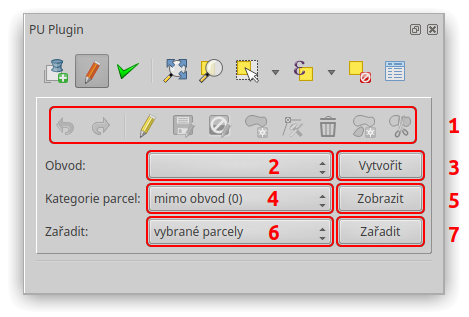
\includegraphics[width=0.55\textwidth]{pictures/editace_gui.png}
\end{figure}

\end{frame}

%------------------------------------------------------------------

\subsection{Kontroly a analýzy}

\begin{frame}

\frametitle{Kontroly a analýzy}

% Kontroly nabízí možnost ověření souladu souboru popisných a geodetických informací.
% Analýzy slouží k provedení výpočtů nutných pro vyhotovení vstupních soupisů nároků vlastníků.

\begin{itemize}
	\item kontroly
	\begin{itemize}
		\item kontrola – obvodem
		\item kontrola – není v SPI
		\item kontrola – není v mapě
		\item kontrola – výměra nad mezní odchylkou
		\item kontrola – bez vlastníka
	\end{itemize}
	\item analýzy
	\begin{itemize}
		\item analýza – měření vzdálenosti
		\item analýza – oceňování podle BPEJ
	\end{itemize}
\end{itemize}

\begin{figure}[ht]
	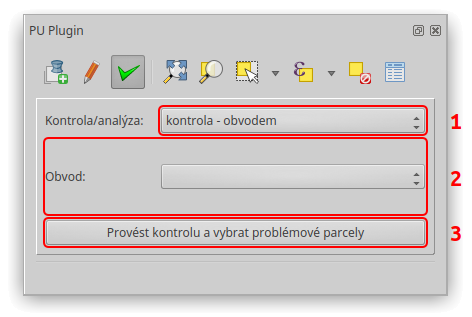
\includegraphics[width=0.55\textwidth]{pictures/ca_gui.png}
\end{figure}

\end{frame}

%------------------------------------------------------------------

\section{Závěr}

\begin{frame}

\frametitle{Závěr}

\begin{itemize}
	\item zdrojový kód
	\begin{itemize}
		\item \url{https://github.com/ctu-geoforall-lab-projects/dp-svoboda-2017}
	\end{itemize}
	\item uživatelský manuál
	\item funkcionalita
	\begin{itemize}
		\item načtení VFK souboru
		\item editace
		\item kontroly a analýzy
	\end{itemize}
	\item instalace přes repositář organizace CTU GeoForAll Lab
	\item další vývoj
	\begin{itemize}
		\item \url{https://github.com/ctu-geoforall-lab/qgis-pu-plugin}
	\end{itemize}
\end{itemize}

\begin{figure}[ht]
	
\includegraphics[width=0.1\textwidth]{pictures/puplugin.png}
\end{figure}

% zásuvný modul testován projektanty pozemkových úprav
% vylepšení poskytovatele dat OGR systému QGIS - 2.18.5
% Zájem projevili i zaměstnanci Státního pozemkového úřadu České republiky, kteří by zásuvný modul rádi používali během programové fáze, ve které se určuje finanční a časová náročnost provedení pozemkových úprav jednotlivých katastrálních území.
% vývoj
% 	- sestavení vlastních nárokových listů
% 	- zvýšení rychlosti kontroly výměra nad mezní odchylkou
% 	- přidání volby symbologie podle listu vlastnictví

\end{frame}

%------------------------------------------------------------------

\begin{frame}

\Huge{\centerline{Děkuji za pozornost.}}

\end{frame}

%------------------------------------------------------------------

\section{Reakce na otázky oponenta}

\begin{frame}

\frametitle{Reakce na otázky oponenta}

Jak se do~atributové tabulky vrstvy PAR zapíší stavební parcely v~katastrálním území s~dvěma číselnými řadami?

\begin{itemize}
	\item sloupec \texttt{\detokenize{DRUH_CISLOVANI_PAR}}
	\begin{itemize}
		\item \texttt{1} – stavební parcela
		\item \texttt{2} – pozemková parcela
	\end{itemize}
	\item atributová tabulka
	\begin{itemize}
		\item \texttt{\detokenize{KMENOVE_CISLO_PAR}} – alias \texttt{KMENOVE C. (PUV.)}
		\item \texttt{\detokenize{PODDELENI_CISLA_PAR}} – alias \texttt{PODDELENI C. (PUV.)}
	\end{itemize}
	\item opraveno v~repositáři pro další vývoj
\end{itemize}

\begin{figure}[ht]
	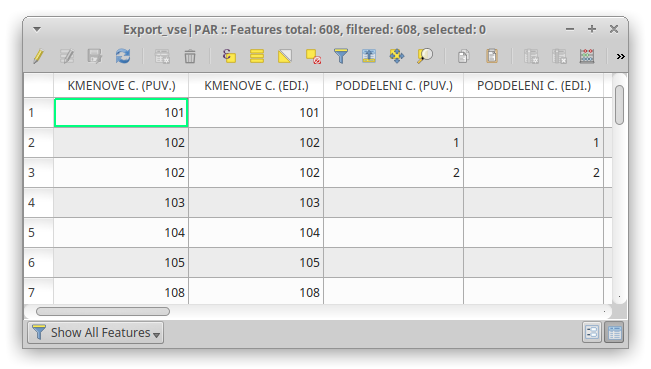
\includegraphics[width=0.85\textwidth]{pictures/nacteni-tabulka.png}
\end{figure}

\end{frame}

%------------------------------------------------------------------

\begin{frame}

\frametitle{Reakce na otázky oponenta}

Bylo by možné použít vytvořený modul i~v~katastrálním území, kde stále existují parcely zjednodušené evidence (např. nedořešené grafické příděly)?

\begin{itemize}
	\item sloupec \texttt{\detokenize{PAR_TYPE}}
	\begin{itemize}
		\item \texttt{PKN} – parcela KN
		\item \texttt{PZE} – parcela ZE
	\end{itemize}
	\item zásuvný modul Georeferencer GDAL
	\item nástroj \textit{Přidat část}
\end{itemize}

\begin{figure}[ht]
	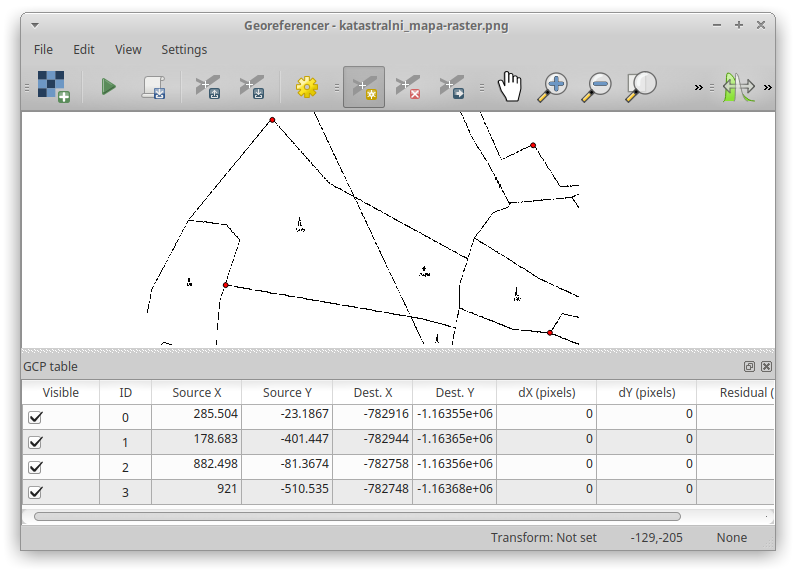
\includegraphics[width=0.6\textwidth]{pictures/georeferencer.png}
\end{figure}

\end{frame}

%------------------------------------------------------------------

\begin{frame}

\frametitle{Reakce na otázky oponenta}

Při určování mezní odchylky ve~výměře vycházíte z~bodu s~nejvyšší hodnotou kódu kvality, nebo z~bodu s~nejnižší přesností (největší základní střední souřadnicovou chybou pro~daný kód kvality)?

\begin{table}[H]
	\fontsize{8}{10}\selectfont
    \begin{tabular}{|l|l|l|}
    	\hline
		\begin{tabular}{@{}l@{}l@{}}
			kód kvality nejméně \\ přesně určeného bodu \\ na~hranici parcely
		\end{tabular} &
		\begin{tabular}{@{}l@{}}
			základní střední \\ souřadnicová chyba [m]
		\end{tabular} &
		mezní odchylka [m\textsuperscript{2}] \\
		\hline
		\hline \texttt{3} & 0.14 & $2$ \\
		\hline \texttt{4} & 0.26 & $0.4*\sqrt{P}+4$ \\
		\hline \texttt{5} & 0.50 & $1.2*\sqrt{P}+12$ \\
		\hline \texttt{6} & 0.21 & $0.3*\sqrt{P}+3$ \\
		\hline \texttt{7} & 0.42 & $0.8*\sqrt{P}+8$ \\
		\hline \texttt{8} & 1.00 & $2.0*\sqrt{P}+20$ \\
		\hline
    \end{tabular} \centering
\end{table}

\begin{itemize}
	\item kde $P$ je větší z~porovnávaných výměr v~metrech čtverečních
	\item opraveno v~repositáři pro další vývoj
\end{itemize}

\end{frame}

%==================================================================
\end{document} 
